% generated by scripts/pkl_to_latex.py
% source PKL : uscan_v1_L6_Ne4_t1_mode-uniform_nmin2_solver-gcg_full_restarts10_iter300_kmax4_tol1em09_U1to20_N20-d03a74da789e.pkl
% scan type  : uscan
% state      : gs
% requires   : \usepackage{pgfplots} \pgfplotsset{compat=1.18}
% colours match the matplotlib PDF (tab10 cycle)
\definecolor{gmeC0}{HTML}{1F77B4}
\definecolor{gmeC1}{HTML}{FF7F0E}
\definecolor{gmeC2}{HTML}{2CA02C}
\definecolor{gmeC3}{HTML}{D62728}
\definecolor{gmeC4}{HTML}{9467BD}
\definecolor{gmeC5}{HTML}{8C564B}
\definecolor{gmeC6}{HTML}{E377C2}
\definecolor{gmeC7}{HTML}{17BECF}

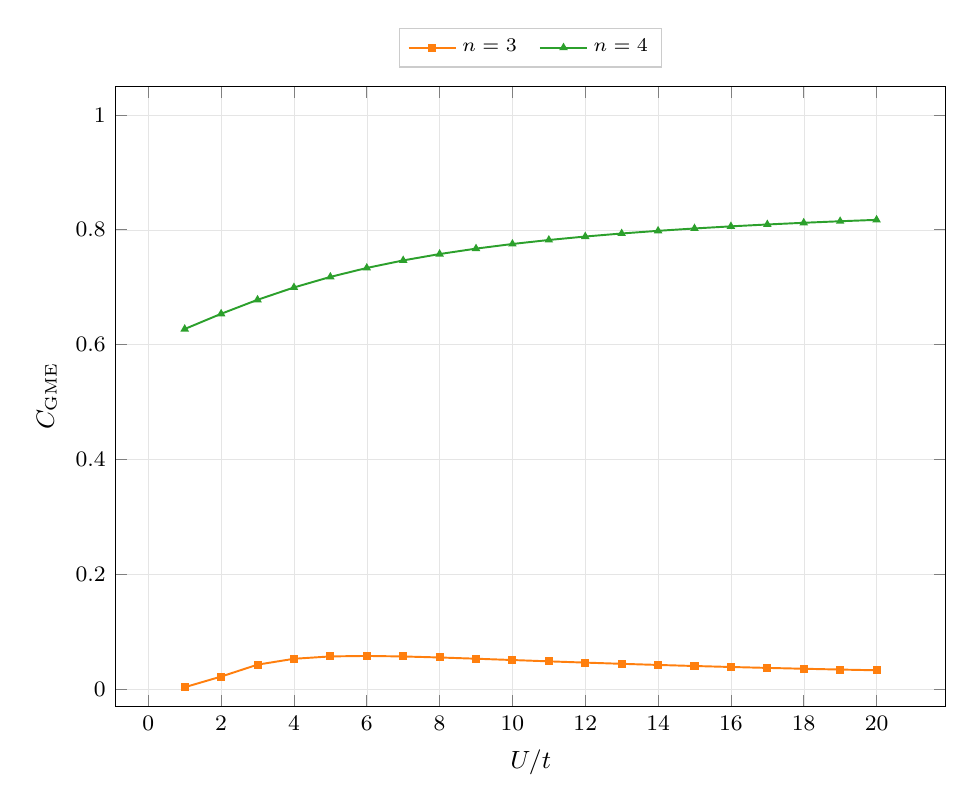
\begin{tikzpicture}
  \begin{axis}[
    width=\columnwidth,
    height=0.78\columnwidth,
    xlabel={$U/t$},
    ylabel={$C_{\mathrm{GME}}$},
    grid=both,
    grid style={line width=.1pt, draw=gray!20},
    tick label style={font=\footnotesize\rmfamily, /pgf/number format/fixed},
    label style={font=\small\rmfamily},
    scaled ticks=false,
    legend style={font=\scriptsize\rmfamily, draw=gray!40, at={(0.5,1.03)}, anchor=south, /tikz/every even column/.append style={column sep=6pt}},
    legend cell align={left},
    legend columns=2,
    ymin=-0.03,
    ymax=1.05,
  ]
    \addplot[color=gmeC1, mark=square*, mark size=1.1pt, line width=0.7pt] coordinates {
        (1,0.003284) (2,0.021825) (3,0.042593) (4,0.05279)
        (5,0.056923) (6,0.057752) (7,0.056848) (8,0.055081)
        (9,0.052923) (10,0.050632) (11,0.048348) (12,0.046139)
        (13,0.044043) (14,0.042074) (15,0.040231) (16,0.038517)
        (17,0.036918) (18,0.035431) (19,0.034048) (20,0.032758)
    };
    \addlegendentry{$n=3$}
    \addplot[color=gmeC2, mark=triangle*, mark size=1.1pt, line width=0.7pt] coordinates {
        (1,0.627051) (2,0.653559) (3,0.677951) (4,0.699417)
        (5,0.717816) (6,0.733389) (7,0.746527) (8,0.757633)
        (9,0.767071) (10,0.775145) (11,0.782102) (12,0.78814)
        (13,0.793417) (14,0.798062) (15,0.802174) (16,0.805838)
        (17,0.80912) (18,0.812074) (19,0.814745) (20,0.817172)
    };
    \addlegendentry{$n=4$}
  \end{axis}
\end{tikzpicture}
